\documentclass{standalone}
\usepackage{../../../../preamble_formulas}

\begin{document}

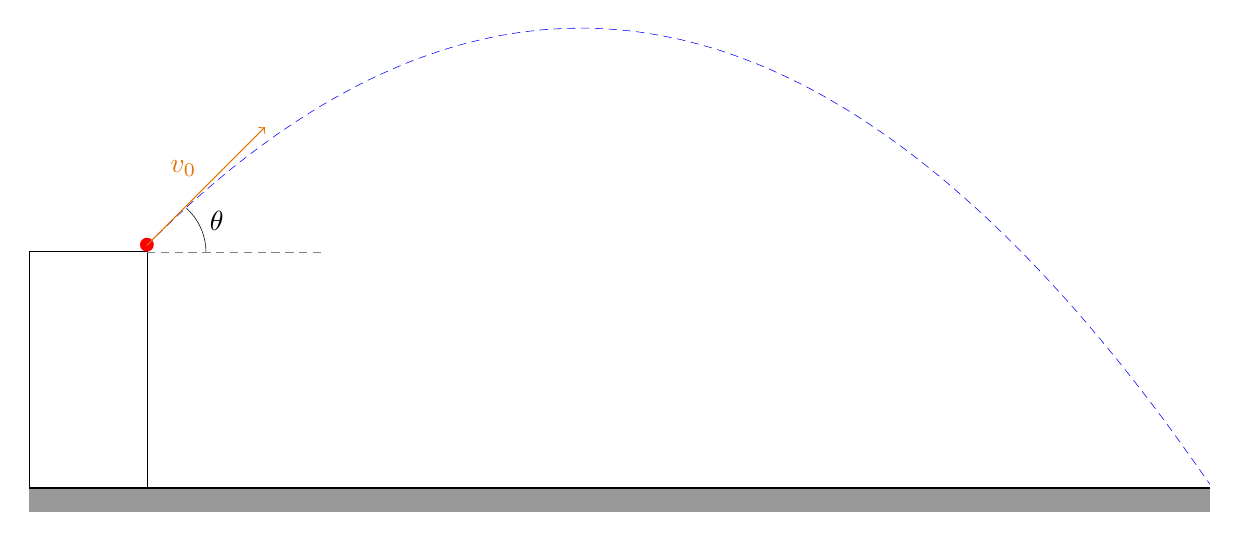
\begin{tikzpicture}[scale=3]

  % ground and rectangle
  \fill [black!40] (0,0) rectangle (5,-0.1);
  \draw[thick] (0,0) -- (5,0);
  \node[rectangle,draw=black,minimum width=1.5cm,minimum height=3cm,anchor=south west] at (0,0){};

  % ball
  \node[circle,fill=red,inner sep=0pt,minimum height=5pt,anchor=south] at (0.5,1){};

  % dashed lines 
  \draw[blue, densely dashed, very thin]   plot[smooth,domain=0.5:5] (\x, {1.03+(\x-0.5)-9.8*(\x-0.5)^2/6^2});
  \draw[gray, densely dashed, very thin] (0.5,1) -- (1.25,1);

  % arc
  \draw[very thin] (0.75,1) arc [start angle=0,end angle=48,x radius=0.25cm,y radius=0.25cm];
  \node[anchor=south west] at (0.725,1.05){$\theta$};

  % arrow
  \draw[->,orange!90!black] (0.5,1+0.0293) -- node[orange!90!black,anchor=south east]{$\vb{v}_0$} (1,1-0.5+1+0.0293);
\end{tikzpicture}

\end{document}